%!TEX root = ../username.tex
\chapter{Genetic Algorithms} \label{ga}

In this project, the melodies generated by the Markov model are used as the initial population for the genetic algorithm.

\section{Fitness Function} \label{ga:fitness}

In several previous papers, the authors discuss the use of interactive fitness functions \cite{papadopoulos_ai_1999} \cite{mcvicar_autoguitartab:_2015}.
With this method, a human listens to the melodies and selects the best from each generation to be used as the parents of the next generation.
This method does well at picking the most pleasing music to human ears, but it requires humans to listen to the music, which is slow and can lead to fatigue on the part of the evaluators.

Rather than rely on humans who may become tired or slightly alter their definition of good music, we want to use an automated fitness function.
Music from the common practice period of Western music, which lasted from the late Baroque period through the Romantic period (~1650-1900), generally followed a complex set of rules regarding harmony, rhythm, and duration.
We could manually define a function that uses some weighted average of each of the many rules, but this approach could be highly error prone and require lots of manual tweaking.

Rather, it is good enough to approximate a fitness function using what we call a surrogate model. % cite a paper on this
Some authors discuss some techniques for fitness functions as applied to music \cite{papadopoulos_ai_1999} \cite{de_freitas_originality_2011} \cite{alfonseca_fitness_2006}.
For example, de Freitas and Guimaraes use a fitness function that penalizes any not outside of the C Major scale, while Papadopoulos and Wiggins use a fitness function that considers several characteristics of the melody, including consecutive intervals, note durations, and contour.
In this project we use an artificial neural network as the surrogate model.
We expect the neural network to pick up on which rules are the most important, altering its weights accordingly.
For this project, we consider eight measures at a time as the input for the neural network.
In our corpus of music, the sixteenth note is most commonly the smallest rhythmic value in a piece of music, so we use $16 * 8 = 128$ input nodes.
Somewhat arbitrarily, we initially use $100$ nodes in a hidden layer.
Through trial and error, the optimal number of hidden layers is $X$ with $Y$ nodes in each hidden layer. % TODO update these to real values
One output node with a value between zero and one gives the neural network's certainty that the provided input is proper, rule following music.
In addition to the samples of ``correct'' music from the corpus, the neural network was also fed completely randomly generated music as examples of ``bad'' music during training.

\section{Mutations} \label{ga:mutate}

There are several natural mutations to consider when working with music.
Two common compositional techniques are inversion and retrograde.
Inversion takes a section of music, generally a couple of measures, and inverts all the intervals, so an interval up becomes the same interval down.
Retrograde reverses the order of one or both of the rhythms and pitches of a section of music.
Retrograde and inverse can also be combined, to yield retrograde-inverse.
Typically, the section is inverted, and the new notes are then read backwards, though some composers, such as Igor Stravinsky, reversed the order of the notes first.
See Figure \ref{fig:p-r-i-ri} for an example of inversion, retrograde, and retrograde-inversion.
These techniques are especially common in twelve tone music, which was developed during the early twentieth century by Arnold Schoenberg, though they can also be found in other types of music. % TODO give examples

\begin{figure}
	\centering
	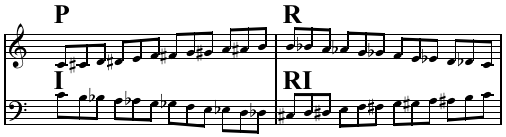
\includegraphics[width=\linewidth]{figures/P-R-I-RI.png} % TODO cite image https://commons.wikimedia.org/wiki/File:P-R-I-RI.png
	\caption{Common  clockwise from the top left: prime (original form), retrograde, inverse, and retrograde-inverse.}
	\label{fig:p-r-i-ri}
\end{figure}

\section{Manipulating Melodies} \label{ga:manip}


